\section{Rails Web Servers} % (fold)
\label{solution:sec:rails_web_servers}
There are many Rails-compatible web servers with distinct philosophies and purposes. Passenger, Thin and Unicorn were targeted for benchmarking, in an effort to determine which is best for each situation. Memory usage and stability are important factors and were taken into account when evaluating each alternative. Apache, Nginx and Cherooke's performance as reverse proxies was also analyzed.

Among the previously introduced web servers, some are missing from this analysis. Ruby's pioneer web server---WEBrick---is left out since it lacks the efficiency to compete with nowadays alternatives. Mongrel, while representing a huge improvement over WEBrick, still lags behind more recently developed web servers as explored in Section~\ref{state:sec:rails_web_servers}, also being excluded from further analysis.

Throughly analyzing the performance, stability and memory usage of up-to-date web server setups was the general goal of the work presented in this section.

\subsection{Development}
Monitoring memory usage is crucial to evaluate the performance of a web server. A web server that consumes less memory is likely to scale better since it can spawn more working processes/threads in the same setup.

There was need for a small utility to measure the memory usage of specified processes over time, providing the ability to configure its refresh interval. It had to be very light not to interfere with the tests, should rely on the operating system's data and preferably output in a easily parsable format. This tool was created and is presented on appendix~\ref{ap:monitor}. It takes a few arguments, namely:
\begin{itemize}
  \item Directory to use when outputting the results;
  \item Refresh interval in seconds (optional, default: 1);
  \item Name of the process(es) to monitor;
\end{itemize}
The utility records each process's memory usage in its own file. For each process, it will record the data in a file entitled \textit{process\_name.process\_pid.csv}. As the name implies, it records the data in the CSV format. Finally, it is compatible with any UNIX system.

This tool was used to measure the memory usage in all benchmarks contained in the following section.

\subsection{Benchmarking}
Ruby has a few highly performant web servers with Passenger, Thin and Unicorn among them. Exchanging web servers in a Rails' setup is not an uncommon activity since improved versions are being frequently released in recent years, as stated in Section~\ref{tech:sec:rails_webservers}.

Regarding this component, benchmarking had four distinct phases. First of all, it was important to evaluate the performance of Apache, Nginx and Cherokee as reverse proxies. After that, the goal was to determine whether Passenger performs better in combination with Apache or Nginx. The third phase would compare Thin's performance to Unicorn's since, as stated on Section~\ref{tech:sec:rails_webservers}, they are developed for similar purposes. All these initial phases would use MRI as the Ruby interpreter. Finally, a more complete benchmark including Passenger, Thin and Unicorn was done, involving multiple quantities of workers and running with MRI and YARV.

For all benchmarks, three distinct pages were used. One \textit{heavy page} filled with dynamic content, a \textit{regular page} with moderate usage of dynamic content and finally a complex but small \textit{API call}. \textit{Escolinhas.pt} was the platform to provide this different types of content.

No database caching solutions were in use. Once again, if more than 1\% of the requests took more than 30 seconds to be replied to the test was considered a failure, as it already surpasses acceptable response times in real world applications. % FIXME: Pôr ref de novo?

\subsubsection{Proxy Performance in a Thin Cluster Environment}
Many Ruby web servers run behind a reverse proxy which buffers the requests, delivers them to the web server and receives the replies, buffering them as well if needed. In this kind of commonly used architecture, they have an important role when it comes to performance.

Thin is a kind of web server that should be paired with a reverse proxy. It is optimized for small requests and fast clients so it needs to rely on the proxy's buffering abilities to offer consistent performance across all kinds of light or heavy content and fast or slow clients.

This benchmark used 4 Thin processes. The only modifications made to its default configuration were related to increasing its request queue, so that it could queue more clients instead of discarding them. This Thin cluster was working behind the 3 aforementioned reverse proxies---Apache, Nginx and Cherooke. The benchmark involved many levels of concurrency, as follows:
\begin{itemize}
  \item 50 requests, 1 concurrent;
  \item 100 requests, 10 concurrent;
  \item 500 requests, 50 concurrent;
  \item 500 requests, 100 concurrent;
  \item 2500 requests, 500 concurrent.
\end{itemize}
The total time to complete each test and the replies \textit{per second} capability of each setup were recorded using the aforementioned tool---\textit{ab}---created by the Apache Foundation\footnote{\url{http://www.apache.org/}}. When using this tool, the user specifies the total amount of requests to be sent and the desired concurrency. It then dispatches all requests to the specified host at the chosen concurrency rate.

The results of this benchmark are presented on table~\ref{tab:reverse_proxy_benchmark}.\\ % FIXME: formatação
\begin{center}
\renewcommand{\arraystretch}{0.85}
\normalsize
\begin{longtable}{c|c|c|c|c|c}
  \caption{Reverse Proxy Benchmark} \label{tab:reverse_proxy_benchmark} \\

  \textbf{Req. / Conc.} & \textbf{Page} & \textbf{Proxy} & \textbf{Requests/s (\#)} & \textbf{Total time (s)} & \textbf{Mem. Usage (B)} \\ \hline 
  \endfirsthead

  \multicolumn{6}{c}%
  {{\bfseries \tablename\ \thetable{} --- continued from previous page}} \\
  \textbf{Req. / Conc.} & \textbf{Page} & \textbf{Proxy} & \textbf{Requests/s (\#)} & \textbf{Total time (s)} & \textbf{Mem. Usage (B)} \\
  \endhead

  \multicolumn{6}{r}{{\tablename\ \thetable{} --- continued on the next page}} \\ \hline
  \endfoot

  \endlastfoot
  
    \multirow{9}{*}{50/1} & \multirow{3}{*}{API} & Cherokee & \textbf{9.96} & \textbf{5.02} & 167553\\\cline{3-6}
     &  & Apache & 9.88 & 5.058 & 200126\\\cline{3-6}
     &  & Nginx & 9.24 & 5.411 & \textbf{121213}\\\cline{2-6}
     & \multirow{3}{*}{Heavy} & Cherokee & \textbf{1.25} & \textbf{39.843} & 171311\\\cline{3-6}
     &  & Apache & 1.22 & 40.887 & 201862\\\cline{3-6}
     &  & Nginx & 1.22 & 41 & \textbf{121506}\\\cline{2-6}
     & \multirow{3}{*}{Regular} & Cherokee & 6.36 & 7.863 & 158716\\\cline{3-6}
     &  & Apache & \textbf{6.88} & \textbf{7.272} & 216544\\\cline{3-6}
     &  & Nginx & 5.99 & 8.341 & \textbf{121325}\\\hline
    \multirow{9}{*}{100/10} & \multirow{3}{*}{API} & Cherokee & 9.76 & 10.246 & 178254\\\cline{3-6}
     &  & Apache & 11.47 & 8.715 & 200734\\\cline{3-6}
     &  & Nginx & \textbf{11.84} & \textbf{8.444} & \textbf{121412}\\\cline{2-6}
     & \multirow{3}{*}{Heavy} & Cherokee & 1.22 & 82.178 & 191255\\\cline{3-6}
     &  & Apache & 2.1 & 47.593 & 215347\\\cline{3-6}
     &  & Nginx & \textbf{2.25} & \textbf{44.495} & \textbf{121666}\\\cline{2-6}
     & \multirow{3}{*}{Regular} & Cherokee & 6.76 & 14.785 & 183319\\\cline{3-6}
     &  & Apache & 6.71 & 14.906 & 200220\\\cline{3-6}
     &  & Nginx & \textbf{12.14} & \textbf{8.236} & \textbf{121402}\\\hline
    \multirow{9}{*}{500/50} & \multirow{3}{*}{API} & Cherokee & 9.6 & 52.108 & 187319\\\cline{3-6}
     &  & Apache & 11.65 & 42.926 & 341887\\\cline{3-6}
     &  & Nginx & \textbf{11.67} & \textbf{42.332} & \textbf{121593}\\\cline{2-6}
     & \multirow{3}{*}{Heavy} & Cherokee & 1.31 & 382.773 & 220144\\\cline{3-6}
     &  & Apache & 2.33 & 214.235 & 356046\\\cline{3-6}
     &  & Nginx & \textbf{2.37} & \textbf{212.427} & \textbf{125128}\\\cline{2-6}
     & \multirow{3}{*}{Regular} & Cherokee & 6.65 & 75.147 & 187706\\\cline{3-6}
     &  & Apache & 12.35 & 40.5 & 342251\\\cline{3-6}
     &  & Nginx & \textbf{12.45} & \textbf{40.173} & \textbf{121625}\\\hline
    \multirow{9}{*}{500/100} & \multirow{3}{*}{API} & Cherokee & 9.53 & 52.474 & 187887\\\cline{3-6}
     &  & Apache & 11.45 & 43.676 & 326127\\\cline{3-6}
     &  & Nginx & \textbf{11.48} & \textbf{43.546} & \textbf{121613}\\\cline{2-6}
     & \multirow{3}{*}{Heavy} & Cherokee & 1.21 & 412.288 & 192303\\\cline{3-6}
     &  & Apache & FAIL & FAIL & 326197\\\cline{3-6}
     &  & Nginx & \textbf{2.45} & \textbf{203.037} & \textbf{127759}\\\cline{2-6}
     & \multirow{3}{*}{Regular} & Cherokee & 6.59 & 75.892 & 191297\\\cline{3-6}
     &  & Apache & 12.48 & 40.065 & 326209\\\cline{3-6}
     &  & Nginx & \textbf{12.54} & \textbf{39.883} & \textbf{121650}\\\hline
    \multirow{9}{*}{2500/500} & \multirow{3}{*}{API} & Cherokee & FAIL & FAIL & 199987\\\cline{3-6}
     &  & Apache & FAIL & FAIL & 342211\\\cline{3-6}
     &  & Nginx & FAIL & FAIL & \textbf{122012}\\\cline{2-6}
     & \multirow{3}{*}{Heavy} & Cherokee & FAIL & FAIL & 199006\\\cline{3-6}
     &  & Apache & FAIL & FAIL & 342472\\\cline{3-6}
     &  & Nginx & FAIL & FAIL & \textbf{127524}\\\cline{2-6}
     & \multirow{3}{*}{Regular} & Cherokee & FAIL & FAIL & 195006\\\cline{3-6}
     &  & Apache & FAIL & FAIL & 340655\\\cline{3-6}
     &  & Nginx & FAIL & FAIL & \textbf{122020}\\
\end{longtable}
\end{center}

On nonexistent concurrency, Cherokee and Apache yielded slightly better results. When concurrency is present and increases, Nginx performs slightly better. On maximum concurrency, however, none was able to cope with the demand. Regarding this last test, Cherokee failed to complete most of the requests. Nginx completed significantly more but most of them also timed out, accounting as a failed test. Apache was able to complete a few requests before becoming unresponsive, but much less than Nginx. Finally, the most impressive remark is that the memory usage of Thin with Nginx is remarkably low and impressively stable, whether it is a light API call or a heavy page. This combination brings an impressive scalability potential for its low memory usage.

\subsubsection{Passenger Performance on Apache/Nginx}
Passenger is different from the previously mentioned web servers. It is not a web server itself but instead acts as module and adds the needed functionality to Apache or Nginx to support web applications written in Ruby. Uncertainty arises when asserting whether Passenger performs better in Apache or Nginx, so a generic benchmark regarding this issue followed.

The test was similar to the one explained in the previous sections. It tested the same request/concurrency combinations, used \textit{ab} to measure the response rate and used the previously mentioned monitoring script to measure the memory usage. It also used 4 Passenger instances. The Passenger-specific configurations were the same on both web servers---Apache and Nginx---and can be seen on table~\ref{tab:passenger4_configuration}.
\begin{table}[h!t]
  \centering
  \caption{Passenger Options and Values}
  \label{tab:passenger4_configuration}
  
  \begin{tabular}{p{0.35\textwidth}|p{0.20\textwidth}}
  
    \textsc{\textbf{Option}} & \textsc{\textbf{Value}} \\ \hline
    Spawn Method & smart \\ \hline
    Maximum Requests & 5000 \\ \hline
    Filesystem Checks Interval & 5 \\ \hline
    Application Spawner Idle Time & 0 \\ \hline
    Pool Idle Time & 1000 \\ \hline
    Maximum Pool Size & 4 \\
  
  \end{tabular}
\end{table}

The results are exhibited on table~\ref{tab:passenger_benchmark}.
\begin{table}[h!t]
  \centering
  \caption{Passenger Benchmark Results on Apache and Nginx}
  \label{tab:passenger_benchmark}
  
  \begin{tabular}{c|c|c|c|c|c}

    \textbf{Req. / Conc.} & \textbf{Page} & \textbf{Web Server} & \textbf{Requests/s (\#)} & \textbf{Total time (s)} & \textbf{Mem. Usage (B)} \\ \hline
    \multirow{6}{*}{50/1} & \multirow{2}{*}{API} & Apache & \textbf{9.37} & \textbf{5.336} & 164429\\\cline{3-6}
     &  & Nginx & 9.1 & 5.496 & \textbf{154437}\\\cline{2-6}
     & \multirow{2}{*}{Heavy} & Apache & \textbf{1.18} & \textbf{42.494} & 154696\\\cline{3-6}
     &  & Nginx & 1.16 & 43.072 & \textbf{142983}\\\cline{2-6}
     & \multirow{2}{*}{Regular} & Apache & 6.24 & 8.017 & 185727\\\cline{3-6}
     &  & Nginx & \textbf{6.36} & \textbf{7.863} & \textbf{154383}\\\hline
    \multirow{6}{*}{100/10} & \multirow{2}{*}{API} & Apache & 12.06 & 8.294 & 207374\\\cline{3-6}
     &  & Nginx & \textbf{12.28} & \textbf{8.146} & \textbf{154453}\\\cline{2-6}
     & \multirow{2}{*}{Heavy} & Apache & \textbf{2.17} & \textbf{45.988} & 168179\\\cline{3-6}
     &  & Nginx & 2.1 & 47.634 & \textbf{156119}\\\cline{2-6}
     & \multirow{2}{*}{Regular} & Apache & \textbf{12.84} & \textbf{7.79} & 181126\\\cline{3-6}
     &  & Nginx & 11.94 & 8.375 & \textbf{149634}\\\hline
    \multirow{6}{*}{500/50} & \multirow{2}{*}{API} & Apache & \textbf{11.63} & \textbf{42.979} & 235130\\\cline{3-6}
     &  & Nginx & 11.53 & 43.383 & \textbf{141376}\\\cline{2-6}
     & \multirow{2}{*}{Heavy} & Apache & FAIL & FAIL & 207180\\\cline{3-6}
     &  & Nginx & \textbf{2.11} & \textbf{237.37} & \textbf{156234}\\\cline{2-6}
     & \multirow{2}{*}{Regular} & Apache & \textbf{12.49} & \textbf{40.043} & 200330\\\cline{3-6}
     &  & Nginx & 12.34 & 40.51 & \textbf{141514}\\\hline
    \multirow{6}{*}{500/100} & \multirow{2}{*}{API} & Apache & FAIL & FAIL & 255006\\\cline{3-6}
     &  & Nginx & \textbf{11.48} & \textbf{43.546} & \textbf{141438}\\\cline{2-6}
     & \multirow{2}{*}{Heavy} & Apache & FAIL & FAIL & 220525\\\cline{3-6}
     &  & Nginx & \textbf{2.1} & \textbf{238.16} & \textbf{156258}\\\cline{2-6}
     & \multirow{2}{*}{Regular} & Apache & FAIL & FAIL & 218195\\\cline{3-6}
     &  & Nginx & \textbf{12.42} & \textbf{40.273} & \textbf{154676}\\\hline
    \multirow{6}{*}{2500/500} & \multirow{2}{*}{API} & Apache & FAIL & FAIL & 238933\\\cline{3-6}
     &  & Nginx & FAIL & FAIL & \textbf{154599}\\\cline{2-6}
     & \multirow{2}{*}{Heavy} & Apache & FAIL & FAIL & 220258\\\cline{3-6}
     &  & Nginx & FAIL & FAIL & \textbf{143133}\\\cline{2-6}
     & \multirow{2}{*}{Regular} & Apache & FAIL & FAIL & 228932\\\cline{3-6}
     &  & Nginx & FAIL & FAIL & \textbf{154699}\\\hline
    \multirow{2}{*}{Total} &  & Apache &  & \textbf{200.941} & 199825\\\cline{2-6}
     &  & Nginx &  & 204.479 & \textbf{150292}\\
  \end{tabular}
\end{table}

When used with Apache, Passenger failed more tests under a rather low concurrency level---100 simultaneous requests---than when used with Nginx, which indicates that this Apache setup has some scalability issues. It should also be noticed that when paired with Nginx, Passenger uses significantly less memory. 

\subsubsection{Thin and Unicorn Performance Comparison}
As mentioned before, Unicorn and Thin are very similar in their goals: they are optimized for small requests and fast clients. However, their philosophies and architecture differ. As mentioned in Section~\ref{tech:sec:rails_webservers}, Thin relies on \textit{EventMachine} for fast I/O processing, using a fast asynchronous event loop. On the other hand, Unicorn forks workers which attend to one client at a time and it relies on the Operating System for many internal tasks like request queuing and worker synchronization. There are many discussions about the performance of these two web servers, becoming an issue worth addressing.

In real world applications, web servers must be ready to serve slow clients and, eventually, heavy pages. Since both web servers are not optimized for these situations, the usage of a reverse proxy is required for request and response buffering purposes.

This benchmark followed the same conditions of the aforementioned ones regarding concurrency, number of processes, test pages and the usage of \textit{ab} to make the measurements. Thin's configuration was the same as before and Unicorn's was very similar to Thin's. Since Nginx yielded excellent results in the previous benchmarks, it was used as both web servers' reverse proxy. The results can be found on table~\ref{tab:thin_unicorn_benchmark}.

\begin{table}[h!t]
  \centering
  \caption{Thin \textit{versus} Unicorn Benchmark Results}
  \label{tab:thin_unicorn_benchmark}
  
  \begin{tabular}{c|c|c|c|c|c}

    \textbf{Req. / Conc.} & \textbf{Page} & \textbf{Web Server} & \textbf{Requests/s (\#)} & \textbf{Total time (s)} & \textbf{Mem. Usage (B)} \\ \hline
    \multirow{6}{*}{50/1} & \multirow{2}{*}{API} & Thin & \textbf{9.24} & \textbf{5.411} & \textbf{121213}\\\cline{3-6}
     &  & Unicorn & 9.17 & 5.45 & 160823\\\cline{2-6}
     & \multirow{2}{*}{Heavy} & Thin & 1.22 & 41 & \textbf{121506}\\\cline{3-6}
     &  & Unicorn & \textbf{1.25} & \textbf{39.849} & 161062\\\cline{2-6}
     & \multirow{2}{*}{Regular} & Thin & 5.99 & 8.341 & \textbf{121325}\\\cline{3-6}
     &  & Unicorn & \textbf{6.89} & \textbf{7.257} & 160845\\\hline
    \multirow{6}{*}{100/10} & \multirow{2}{*}{API} & Thin & 11.84 & 8.444 & \textbf{121412}\\\cline{3-6}
     &  & Unicorn & \textbf{12.22} & \textbf{8.182} & 160828\\\cline{2-6}
     & \multirow{2}{*}{Heavy} & Thin & 2.25 & 44.495 & \textbf{121666}\\\cline{3-6}
     &  & Unicorn & \textbf{2.28} & \textbf{43.832} & 161035\\\cline{2-6}
     & \multirow{2}{*}{Regular} & Thin & 12.14 & 8.236 & \textbf{121402}\\\cline{3-6}
     &  & Unicorn & \textbf{12.46} & \textbf{8.023} & 160865\\\hline
    \multirow{6}{*}{500/50} & \multirow{2}{*}{API} & Thin & \textbf{11.67} & \textbf{42.332} & \textbf{121593}\\\cline{3-6}
     &  & Unicorn & 11.62 & 43.013 & 160919\\\cline{2-6}
     & \multirow{2}{*}{Heavy} & Thin & \textbf{2.37} & \textbf{212.427} & \textbf{125128}\\\cline{3-6}
     &  & Unicorn & 2.31 & 216.525 & 161113\\\cline{2-6}
     & \multirow{2}{*}{Regular} & Thin & \textbf{12.45} & \textbf{40.173} & \textbf{121625}\\\cline{3-6}
     &  & Unicorn & 12.44 & 40.207 & 160955\\\hline
    \multirow{6}{*}{500/100} & \multirow{2}{*}{API} & Thin & \textbf{11.48} & \textbf{43.546} & \textbf{121613}\\\cline{3-6}
     &  & Unicorn & 11.46 & 43.618 & 160997\\\cline{2-6}
     & \multirow{2}{*}{Heavy} & Thin & \textbf{2.45} & \textbf{203.037} & \textbf{127759}\\\cline{3-6}
     &  & Unicorn & 2.3 & 217.513 & 161207\\\cline{2-6}
     & \multirow{2}{*}{Regular} & Thin & 12.54 & 39.883 & \textbf{121650}\\\cline{3-6}
     &  & Unicorn & \textbf{12.65} & \textbf{39.516} & 161027\\\hline
    \multirow{6}{*}{2500/500} & \multirow{2}{*}{API} & Thin & FAIL & FAIL & \textbf{122012}\\\cline{3-6}
     &  & Unicorn & FAIL & FAIL & 161045\\\cline{2-6}
     & \multirow{2}{*}{Heavy} & Thin & FAIL & FAIL & \textbf{127524}\\\cline{3-6}
     &  & Unicorn & FAIL & FAIL & 161193\\\cline{2-6}
     & \multirow{2}{*}{Regular} & Thin & FAIL & FAIL & \textbf{122020}\\\cline{3-6}
     &  & Unicorn & FAIL & FAIL & 161089\\\hline
    \multirow{2}{*}{Total} &  & Thin &  & \textbf{697.325} & \textbf{122324}\\\cline{2-6}
     &  & Unicorn &  & 712.985 & 160973\\
  \end{tabular}
\end{table}

Unicorn's performance is very similar to Thin's. Thin was slightly faster in total while using less memory so it yields a very slim advantaged on the performed benchmarks.

\subsubsection{Ruby Web Servers Benchmark}
The previous benchmarks addressed specific questions that the Ruby community has. The current one, however, aims at exploring all alternatives in the same environment. The results obtained for previous benchmarks narrow down possible alternatives, allowing a complete yet simple benchmark. 

Nginx was used as the reverse proxy for Thin and Unicorn. It was also used as the primary web server where Passenger was docked. As seen on the previous benchmarks, it yields very similar performance to Apache and Cherokee while using less memory.

Similarly to real applications, more processes were used as well. Instead of the 4 workers used in the previous benchmarks, this test contempted 30 and 60 workers. The aforementioned developed script was used to record the memory usage in all tests. The test pages were also the same as the ones used on the previous benchmarks.

In this benchmark, however, the measurement tool was~\textit{autobench}~\footnote{\url{http://www.xenoclast.org/autobench/}}, a wrapper around on HP's~\textit{httperf}~\footnote{\url{http://www.hpl.hp.com/research/linux/httperf/}}. Instead of continuously dumping requests to the target host like \textit{ab} does, \textit{autobench} runs a number of times against the specified host(s), increasing the number of requested connections \textit{per second} on each iteration. Then it tries to find the highest request rate in which the web server remains stable and aims at maintaining that rate for the remaining simulation time, which is defined by the user.

The first round of tests was made using Ruby 1.8. The results for the \textit{heavy page} filled with dynamic content are presented on figure~\ref{fig:page1_autobench_ruby18_results}.
\begin{figure}[h!t]
  \centering
    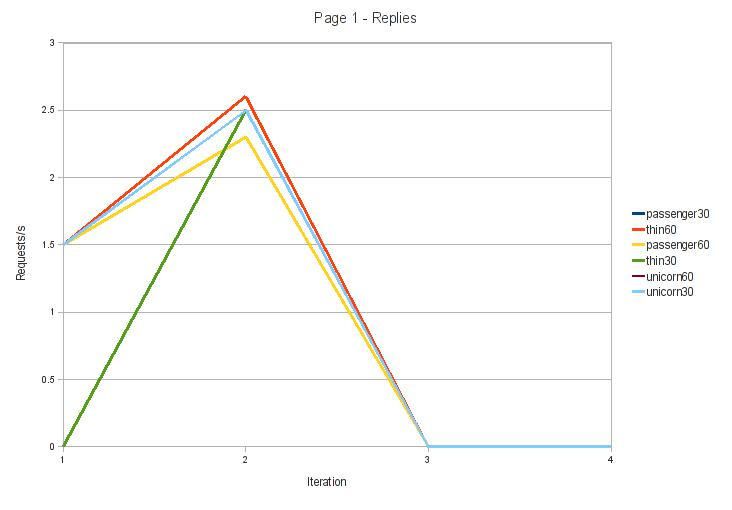
\includegraphics[width=0.95\textwidth]{results_autobench_replies_homepage_ruby18}
    \caption{Autobench Results on the Heavy Page (Ruby 1.8)} \label{fig:page1_autobench_ruby18_results}
\end{figure}

The test tool, \textit{autobench}, was unable to find a stable request rate on this page. All web servers behaved similarly poor. 

As for the \textit{regular page} with moderate usage of dynamic content, the results can be found on figure~\ref{fig:page2_autobench_ruby18_results}.
\begin{figure}[h!t]
  \centering
    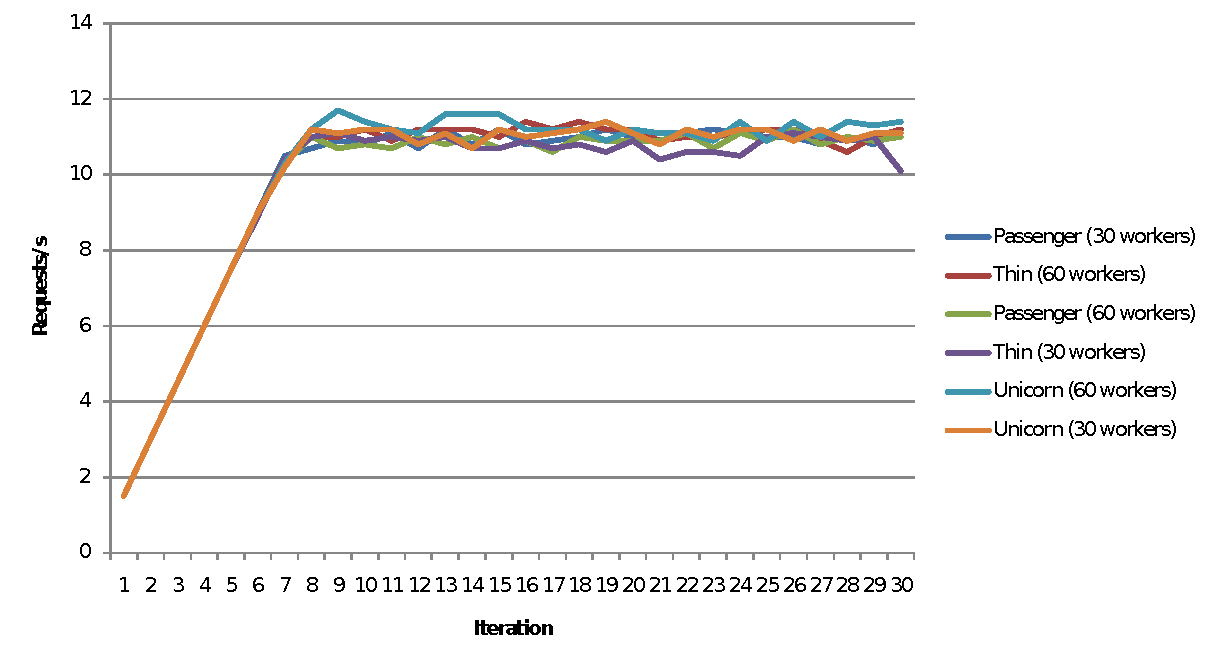
\includegraphics[width=0.95\textwidth]{results_autobench_replies_portal_ruby18}
    \caption{Autobench Results on the Regular Page (Ruby 1.8)} \label{fig:page2_autobench_ruby18_results}
\end{figure}

On this test all web servers were able to consistently serve requests, stabilizing at a rate of 10-12 requests \textit{per second}. Although all had very similar performances, Unicorn with 60 workers consistently yielded slightly better results.

Finally, regarding the complex but small \textit{API call}, the results are exhibited on figure~\ref{fig:page3_autobench_ruby18_results}.
\begin{figure}[h!t]
  \centering
    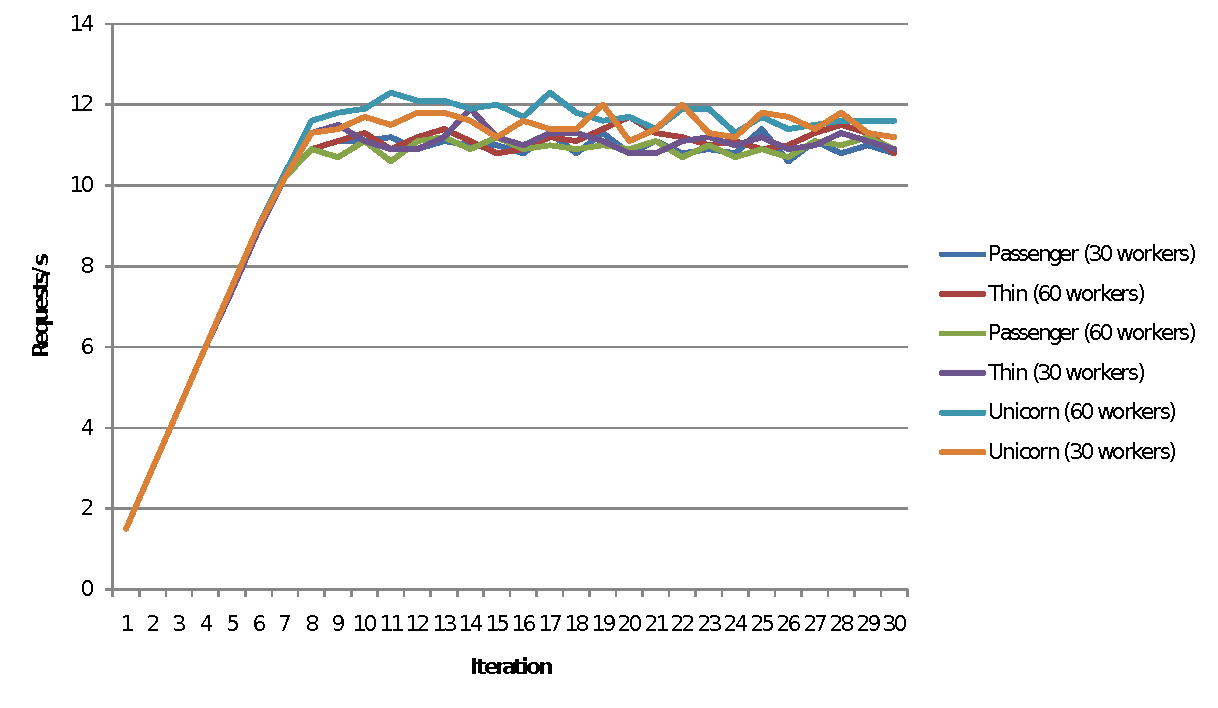
\includegraphics[width=0.95\textwidth]{results_autobench_replies_publication_ruby18}
    \caption{Autobench Results on the API Call (Ruby 1.8)} \label{fig:page3_autobench_ruby18_results}
\end{figure}

Once again, all web servers were able to maintain a stable request rate, which was around 10-13. Unicorn, both with 30 and 60 workers, seems to have a slight performance advantage over its competitors.

The second round was made using Ruby 1.9 on exactly the same pages. The results for the \textit{heavy page} filled with dynamic content can be seen on figure~\ref{fig:page1_autobench_ruby19_results}.
\begin{figure}[h!t]
  \centering
    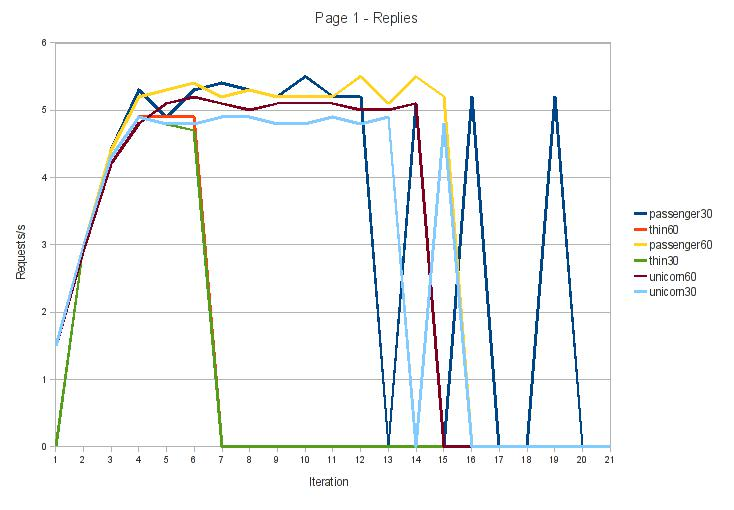
\includegraphics[width=0.95\textwidth]{results_autobench_replies_homepage_ruby19}
    \caption{Autobench Results on the Heavy Page (Ruby 1.9)} \label{fig:page1_autobench_ruby19_results}
\end{figure}

All web servers have shown extreme improvements after switching to YARV on this page. Most of them were stable through 15-16 iterations instead of a single one and the response rate increased from 2,5 to 4,5-5,5. Thin is the most notable exception, loosing stability after 6 iterations. However, it still represents a remarkable improvement over the previous tests with MRI.

As for the \textit{regular page} with moderate usage of dynamic content, the results are presented on figure~\ref{fig:page2_autobench_ruby19_results}.
\begin{figure}[h!t]
  \centering
    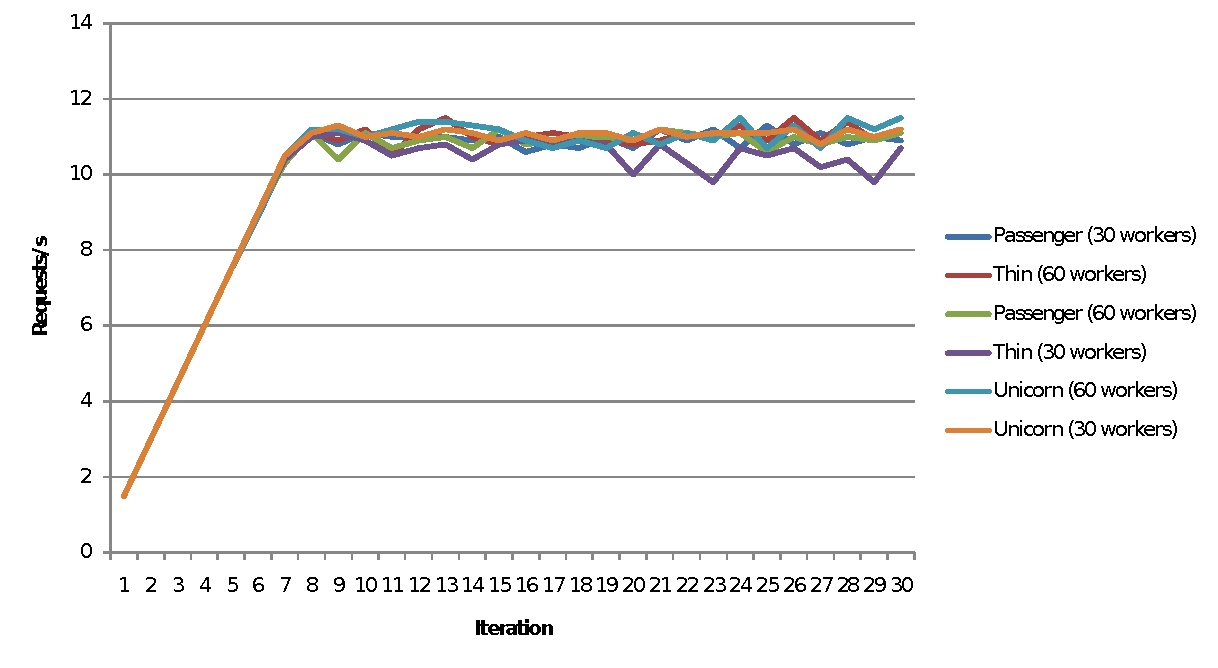
\includegraphics[width=0.95\textwidth]{results_autobench_replies_portal_ruby19}
    \caption{Autobench Results on the Regular Page (Ruby 1.9)} \label{fig:page2_autobench_ruby19_results}
\end{figure}

All web servers performed similarly on this test. The results were also very similar to the same test with Ruby 1.8, mainly due to the fact that this page is relatively light on Ruby code.

Finally, regarding the complex but small \textit{API call}, the results can be found on figure~\ref{fig:page3_autobench_ruby19_results}.
\begin{figure}[h!t]
  \centering
    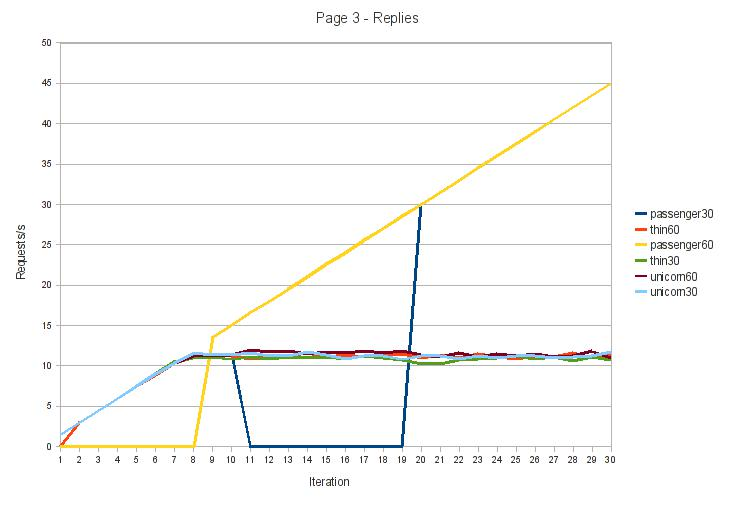
\includegraphics[width=0.95\textwidth]{results_autobench_replies_publication_ruby19}
    \caption{Autobench Results on the API Call (Ruby 1.9)} \label{fig:page3_autobench_ruby19_results}
\end{figure}

Once again, the results are very similar to those found on the same test with Ruby 1.8. Passenger's behavior is not consistent because its application handler segmentation faults on this specific test---complex \textit{API call} on Ruby 1.9 with 30 and 60 workers---which is possibly related with shared resource access among workers.

Table~\ref{tab:web_server_memory_usage} exhibits the average memory usage throughout the test. A few conclusions can be drawn from the memory usage data. Firstly, Thin always uses less memory than the other web servers. Passenger's memory usage with 30 workers is similar to when it is using 60 workers, which is very high when compared to the others. Finally, using Ruby 1.9 generally causes web servers to use less memory.
\begin{table}[h!t]
  \centering
  \caption{Web Server Memory Usage}
  \label{tab:web_server_memory_usage}
  
  \begin{tabular}{l|c|c|c|c|c|c}

     & \multicolumn{2}{c|}{\textbf{\textsc{Heavy Page}}} & \multicolumn{2}{c|}{\textbf{\textsc{Regular Page}}} & \multicolumn{2}{c}{\textbf{\textsc{API Call}}} \\ \hline
     & \textbf{Ruby 1.8} & \textbf{Ruby 1.9} & \textbf{Ruby 1.8} & \textbf{Ruby 1.9} & \textbf{Ruby 1.8} & \textbf{Ruby 1.9} \\ \hline
    \textbf{Thin (30)} & 3041 & 2868 & 3018 & 2802 & 2984 & 2849 \\ \hline
    \textbf{Unicorn (30)} & 3463 & 3556 & 3461 & 3354 & 3461 & 3442 \\ \hline
    \textbf{Passenger (30)} & 7794 & 6920 & 7661 & 6650 & 7666 & 6486 \\ \hline
    \textbf{Thin (60)} & 7214 & 6721 & 6993 & 6206 & 6995 & 6488 \\ \hline
    \textbf{Unicorn (60)} & 6808 & 6878 & 6804 & 6566 & 6803 & 6684 \\ \hline
    \textbf{Passenger (60)} & 7798 & 6921 & 7771 & 6687 & 7771 & 8045 \\
  \end{tabular}
\end{table}

After an exhaustive analysis of web server performance, scalability and memory usage, one can conclude that the performance differences between each alternative are very small. The area of more impact is memory usage where Thin yields the best results, closely followed by Unicorn. Using Ruby 1.9, however, induces a significant improvement in the results regarding the response rate ability and the stability of all web servers. This difference is clearly noticeable in the heaviest test of the benchmark, where most web servers have shown a $\pm$200\% increase in the response rate and $\pm$1500\% increase in successfully completed iterations.

Most of the tests have shown small to no improvements when doubling the number of workers from 30 to 60. The main bottleneck is related to the nonexistence of a memory object caching system, so increasing the workers had no effect on performance. In fact, the difference between the results of this benchmark and the previously shown ones, with only 4 workers, is remarkably small. Database caching should be in use to precisely determine the difference between having 30 and 60 workers on the aforementioned dual-core machine.

\subsection{Tweaking}
Tweaking a web server's configuration is important to fine-tune its performance. All the examined components are highly configurable and changing some settings can provoke a positive or negative impact in performance.

Apache supports two completely different MPM models: a prefork MPM, which forks a number of identical Apache processes and a worker MPM, which creates multiple threads. The prefork model is generally more effective on systems with one or two processing units where the operating systems is better geared toward time slicing between multiple processes. When more CPUs are available, the worker model will probably be more effective. There are also important settings to address like, for instance, defining the maximum number simultaneous connections that Apache can handle using \text{MaxClients} and setting the minimum and maximum number of spare threads/processes.

Unlike Apache, Nginx does not rely on threads nor processes to handle requests. Using a philosophy very similar to Thin's, it aims at solving the C10K problem~\footnote{\url{http://www.kegel.com/c10k.html}} by using an event-driven asynchronous architecture. Nginx supports various event models for handling connections which are optimized for certain situations and operating systems. The user must be certain that it is using the correct one for his system. One of the most efficient models---\textit{epool}---is only supported on Linux systems running a kernel in at least version 2.6, for instance.

Similarly to Apache's worker MPM, Cherokee is a threaded web server. However, it relies on the operating system for request queuing so it also supports many polling methods which are optimized for specific systems, like \textit{epoll}. The amount of threads can and should also be configured specifically for each application and machine.

Thin itself is not as configurable as the previously mentioned web servers. However, there are important settings like, for instance, the maximum number of connections, that can be fine-tuned. As mentioned on Section~\ref{tech:sec:rails_webservers}, Thin recently became capable of operating in a threaded manner by having a background pool of threads, despite its ``single process single thread'' philosophy. The following section will present a benchmark on this option.

Passenger has a significant amount of configuration options. One of the most important is the process spawning method. Setting it to ``smart'' yields the best results, according to its development team. However, it can cause incompatibilities with some \textit{gems}. The developers must test each system and see if this spawning method is suitable or not. Other interesting options include the number of requests interval in which an application process is restarted, useful for when an application has memory leaks.

Unicorn is a very configurable web server. Its configuration is written in Ruby and there is the possibility to hook into many parts of the start and execution processes. Among all options, there is one that is particularly interesting since it can change the size of the buffers which send and receive TCP data. These can be configured to match the kernel ones---defined by \textit{sysctl}---for optimal performance.

\subsubsection{Thin Performance with Threading Enabled}
Thin recently started to offer an option which, when activated, will cause requests to be dispatched to a background pool of 20 threads. This slightly contradicts its initial ``single process single thread'' philosophy, though it still relies on an asynchronous event loop in each thread.

A benchmark comparing Thin's performance when threading is enabled or disabled was made using the three previously mentioned pages. Similarly to the initial benchmarks, 4 workers were used in each test and, like the initial benchmarks, \textit{ab} as used to conduct each test. The results are exhibited on table~\ref{tab:thin_threaded_benchmark}.

\begin{table}[h!t]
  \centering
  \caption{Thin with Threading Benchmark Results}
  \label{tab:thin_threaded_benchmark}
  
  \begin{tabular}{c|c|c|c|c|c}

    \textbf{Req. / Conc.} & \textbf{Page} & \textbf{Web Server} & \textbf{Requests/s (\#)} & \textbf{Total time (s)} & \textbf{Mem. Usage (B)} \\ \hline
    \multirow{6}{*}{50/1} & \multirow{2}{*}{API} & Thin & \textbf{9.24} & \textbf{5.411} & \textbf{121213}\\\cline{3-6}
     &  & Thin(threaded) & 7.5 & 6.665 & 126491\\\cline{2-6}
     & \multirow{2}{*}{Heavy} & Thin & \textbf{1.22} & \textbf{41} & \textbf{121506}\\\cline{3-6}
     &  & Thin(threaded) & 0.91 & 55.221 & 128809\\\cline{2-6}
     & \multirow{2}{*}{Regular} & Thin & \textbf{5.99} & \textbf{8.341} & \textbf{121325}\\\cline{3-6}
     &  & Thin(threaded) & 4.67 & 10.711 & 126954\\\hline
    \multirow{6}{*}{100/10} & \multirow{2}{*}{API} & Thin & \textbf{11.84} & \textbf{8.444} & \textbf{121412}\\\cline{3-6}
     &  & Thin(threaded) & 11.81 & 8.465 & 128097\\\cline{2-6}
     & \multirow{2}{*}{Heavy} & Thin & \textbf{2.25} & \textbf{44.495} & \textbf{121666}\\\cline{3-6}
     &  & Thin(threaded) & 1.84 & 54.468 & 133241\\\cline{2-6}
     & \multirow{2}{*}{Regular} & Thin & \textbf{12.14} & \textbf{8.236} & \textbf{121402}\\\cline{3-6}
     &  & Thin(threaded) & 11.73 & 8.527 & 128709\\\hline
    \multirow{6}{*}{500/50} & \multirow{2}{*}{API} & Thin & \textbf{11.67} & \textbf{42.332} & \textbf{121593}\\\cline{3-6}
     &  & Thin(threaded) & 11.47 & 43.605 & 129938\\\cline{2-6}
     & \multirow{2}{*}{Heavy} & Thin & \textbf{2.37} & \textbf{212.427} & \textbf{125128}\\\cline{3-6}
     &  & Thin(threaded) & FAIL & FAIL & 152066\\\cline{2-6}
     & \multirow{2}{*}{Regular} & Thin & \textbf{12.45} & \textbf{40.173} & \textbf{121625}\\\cline{3-6}
     &  & Thin(threaded) & 11.9 & 42.005 & 130860\\\hline
    \multirow{6}{*}{500/100} & \multirow{2}{*}{API} & Thin & 11.48 & 43.546 & \textbf{121613}\\\cline{3-6}
     &  & Thin(threaded) & \textbf{11.6} & \textbf{43.111} & 130082\\\cline{2-6}
     & \multirow{2}{*}{Heavy} & Thin & \textbf{2.45} & \textbf{203.037} & \textbf{127759}\\\cline{3-6}
     &  & Thin(threaded) & FAIL & FAIL & 139153\\\cline{2-6}
     & \multirow{2}{*}{Regular} & Thin & \textbf{12.54} & \textbf{39.883} & \textbf{121650}\\\cline{3-6}
     &  & Thin(threaded) & 11.68 & 42.818 & 130909\\\hline
    \multirow{6}{*}{2500/500} & \multirow{2}{*}{API} & Thin & FAIL & FAIL & \textbf{122012}\\\cline{3-6}
     &  & Thin(threaded) & FAIL & FAIL & 130558\\\cline{2-6}
     & \multirow{2}{*}{Heavy} & Thin & FAIL & FAIL & \textbf{127524}\\\cline{3-6}
     &  & Thin(threaded) & FAIL & FAIL & 134980\\\cline{2-6}
     & \multirow{2}{*}{Regular} & Thin & FAIL & FAIL & \textbf{122020}\\\cline{3-6}
     &  & Thin(threaded) & FAIL & FAIL & 131290\\
  \end{tabular}
\end{table}

Threaded Thin actually performs worse in these test pages. It uses slightly more memory and generally needs a small amount of extra time to complete each test. Threads have an associated overhead, mainly related to the spawning process and the context switches they provoke. Since Thin is based on a really fast asynchronous loop, it is likely that this processing overhead is, in this case, slowing the web server down overall.


\subsection{Section Overview}
This section exhibited and explained the work concerning Rails web servers. Regarding development, a simple yet powerful memory usage monitoring script was created. Benchmarking, however, had many phases. First of all, proxy performance involving Apache, Nginx and Cherooke was analyzed. The performance of all three was very similar, but Nginx used considerably less memory. Then, Passenger's performance on Apache and Nginx was compared. While having a similar performance across the mentioned web servers, Passenger was more scalable, more stable and used less memory under Nginx. After that, Thin and Unicorn were compared, where Thin performed slightly better while, once again, using less memory. Finally, a more complete benchmark involving Thin, Unicorn, Passenger, Nginx and different Ruby versions was made. All web servers yielded similar results, with Unicorn performing slightly better and Thin maintaining its low memory consumption. Switching from MRI to YARV, however, had a huge positive impact on all web server's performance, mainly noticed on the heaviest test. Finally, concerning tweaking, some web server options were presented and explained. Enabling threads in Thin was one of the options explored, though no performance benefits were detected.

The results obtained during all the benchmark analysis allowed to complete the general goal initially stated. Nginx poses as the best performing reverse proxy, Unicorn yields slightly better performance results under high-load and Thin consistently consumes less memory. However, these differences very scarce.
